%*****************************************
% Lab 03: Arithmetic Operations
%*****************************************
\chapter{Arithmetic Operations}\label{arith}

\section{Purpose}

This lab develops an arithmetic unit that includes eight different arithmetic functions using \LE library items. This device will eventually be used as part of the \acf{ALU} in Lab \ref{alu}. This device will have two inputs, labeled \textit{A} and \textit{B}, and will output the following calculations.

\begin{enumerate}
	\item $ -1 $
	\item $ A-1 $
	\item $ A+B $
	\item $ A-B $
	\item $ AB-1 $
	\item $ AB'-1 $
	\item $ A+A $
	\item $ A+1 $
\end{enumerate}

\section{Procedure}

Start a new \LE project and create a subcircuit named \lstinline[columns=fixed]|arithmetic| that will eventually contain the entire arithmetic unit. Begin the build by adding eight devices in the subcircuit as in Figure \ref{fig:arith-01}. \textit{Notes: exact device placement is not important at this point since they can be repositioned as necessary; however, they should be in the correct order on the subcircuit. Also, all of the devices, inputs, and outputs need to be set for eight data bits in the properties panel.} 

\begin{figure}[H]
	\centering
	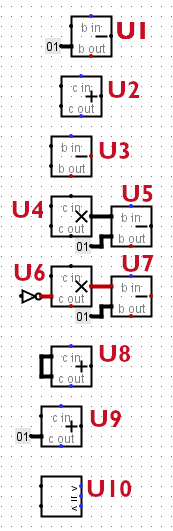
\includegraphics[width=3cm]{gfx/arith-01}
	\caption{Placing the Arithmetic Components}
	\label{fig:arith-01}
\end{figure}

Here are the devices in Figure \ref{fig:arith-01}. \textit{Note: the device numbers were added to the illustration as an aid for the following discussion; they will not be present in the \LE subcircuit.}

\begin{itemize}
	\item U1-Subtractor (\textit{Arithmetic} library). This device subtracts the bottom input from the top input on its east side and sends the result to the output on its west side.
	\item Constant (\textit{Wiring} library). Subtractor \textit{U1} is intended to supply the \textit{A-1} output and the ``01'' on its bottom input is a constant used in this calculation. It should be placed near the bottom input for subtractor \textit{U1} and its properties set for Facing: East, Data Bits: 8, Value: 0x1 (this means hexadecimal 1).
	\item U2-Adder (\textit{Arithmetic} library). This device adds the top and bottom inputs on its east side and sends the result to the output on its west side.
	\item U3-Subtractor (\textit{Arithmetic} library). This device subtracts the bottom input from the top input on its east side and sends the result to the output on its west side.
	\item U4-Multiplier (\textit{Arithmetic} library). This device multiplies the top and bottom inputs on its east side and sends the result to the output on its west side.
	\item U5-Subtractor (\textit{Arithmetic} library). This device is connected to multiplier U4 output and is intended to subtract one from its product.
	\item Constant (\textit{Wiring} library). Because subtractor U5 is designed to subtract one from the product of U4, the ``01'' on its bottom input is a constant. It should be placed near the bottom input and its properties set for Facing: East, Data Bits: 8, Value: 0x1 (this means hexadecimal 1).
	\item U6-Multiplier (\textit{Arithmetic} library). This device multiplies the top and bottom inputs on its east side and sends the result to the output on its west side.
	\item Not Gate (\textit{Gates} library). This is placed near the bottom input of multiplier U6 in order to negate that input.
	\item U7-Subtractor (\textit{Arithmetic} library). This device is connected to multiplier U6 output and is intended to subtract one from its product.
	\item Constant (\textit{Wiring} library). Because subtractor U7 is designed to subtract one from the product of U6, the ``01'' on its bottom input is a constant. It should be placed near the bottom input and its properties set for Facing: East, Data Bits: 8, Value: 0x1 (this means hexadecimal 1).	
	\item U8-Adder (\textit{Arithmetic} library). This device is designed to output the value of $ A+A $ so the two inputs on its east side are tied together. The result is sent to the output on its west side.
	\item U9-Adder (\textit{Arithmetic} library). This device adds the top and bottom inputs on its east side and sends the result to the output on its west side.
	\item Constant (\textit{Wiring} library). Adder \textit{U9} is intended to supply the \textit{A+1} output and the ``01'' on its bottom input is a constant. It should be placed near the bottom input for adder \textit{U9} and its properties set for Facing: East, Data Bits: 8, Value: 0x1 (this means hexadecimal 1).	
	\item U10-Comparator (\textit{Arithmetic} library). A comparator compares the two inputs on its east side. If the top input is greater than the bottom input then output ``$ > $'' will go high. If the top and bottom inputs are equal then output ``$ = $'' will go high. If the top input is less than the bottom input then output ``$ < $'' will go high.
\end{itemize}

The next step is to place all of the inputs and outputs. Figure \ref{fig:arith-02} shows where those items should go and the label for each item. Note: exact placement is not important since they can be repositioned. The \textit{Radix} property for each of the inputs and outputs should be set to ``Hexadecimal.'' The \textit{Data Bits} property should be set as follows.

\begin{itemize}
	\item CI: 1
	\item A: 8
	\item B: 8
	\item ArOut: 8
	\item CO: 1
	\item Cmp: 1
\end{itemize}

\begin{figure}[H]
	\centering
	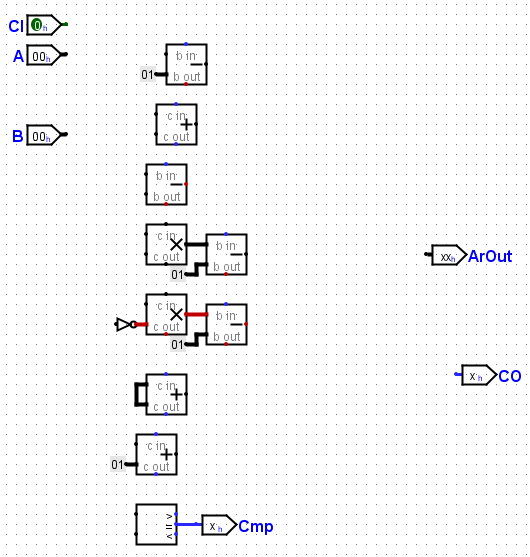
\includegraphics[width=\maxwidth{.95\linewidth}]{gfx/arith-02}
	\caption{Arithmetic Inputs and Outputs}
	\label{fig:arith-02}
\end{figure}

This circuit uses a Multiplexer (\textit{Plexers} library) to select which device's output to connect to \textit{ArOut}. A multiplexer is a digital logic workhorse that is found in many circuits, including \acp{CPU}. It is designed to switch a selected input to the output while ignoring all other input ports. In Figure \ref{fig:arith-03}, two multiplexers have been placed in the circuit. The top multiplexer will select one of eight inputs coming from the eight arithmetic devices to connect to \textit{ArOut}. The bottom multiplexer will connect the carry out signal from the selected arithmetic device to the \textit{CO} output. Also notice that the bottom multiplexer has a constant zero wired to input port zero. 

\begin{figure}[H]
	\centering
	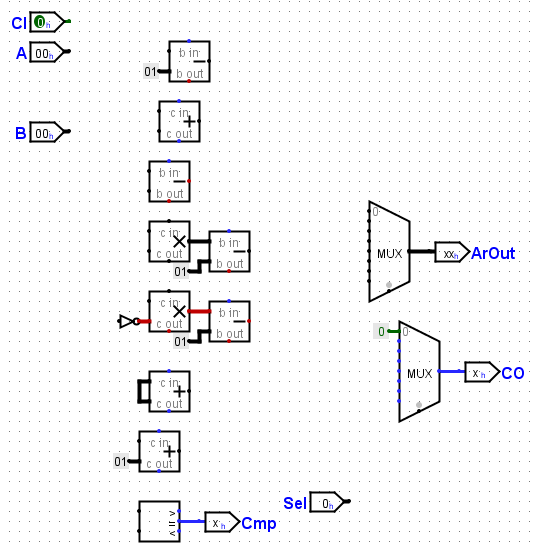
\includegraphics[width=\maxwidth{.95\linewidth}]{gfx/arith-03}
	\caption{Placing the Multiplexers}
	\label{fig:arith-03}
\end{figure}

The next step is to wire inputs \textit{A} and \textit{B} to each of the devices, as shown in Figure \ref{fig:arith-04}. Then the outputs of each device is wired to an appropriate port in the top multiplexer. This is not particularly challenging, but be careful to avoid crossed wires. 

\begin{figure}[H]
	\centering
	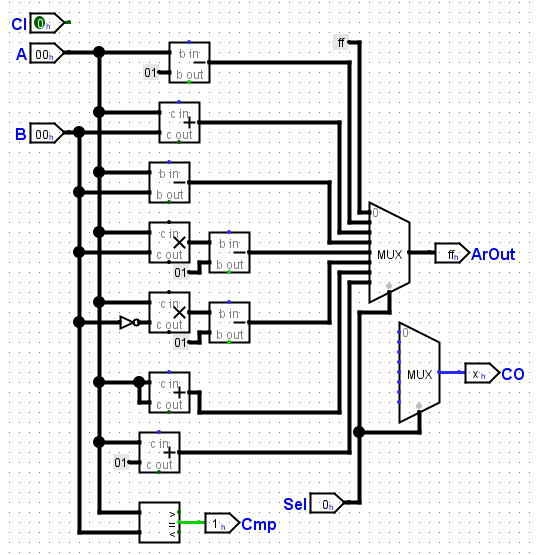
\includegraphics[width=\maxwidth{.95\linewidth}]{gfx/arith-04}
	\caption{Wiring the Data Inputs and Outputs}
	\label{fig:arith-04}
\end{figure}

Figure \ref{fig:arith-04} shows the completed subcircuit with wires connecting \textit{CI} to each device and then the devices wired to the appropriate port on the bottom multiplexer.

Notice that input zero on the top multiplexer is wired to a constant \textit{ff}. That is the two's complement of negative one so that port will always transmit negative one, as in the specification sheet. 

\begin{figure}[H]
	\centering
	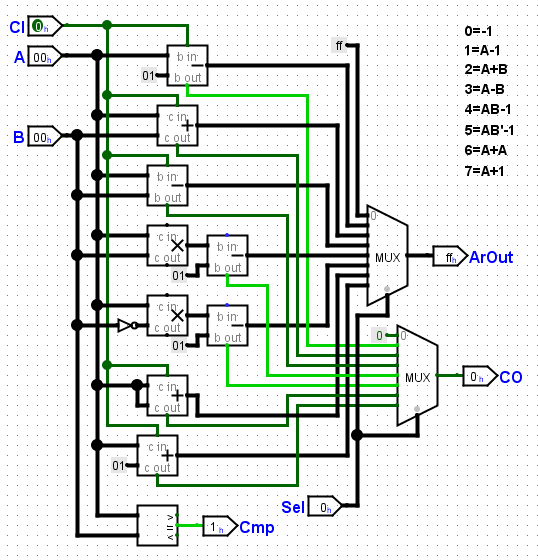
\includegraphics[width=\maxwidth{.95\linewidth}]{gfx/arith-05}
	\caption{Arithmetic Final Circuit}
	\label{fig:arith-05}
\end{figure}

Finally, the \lstinline[columns=fixed]|main| circuit is completed by dropping the \lstinline[columns=fixed]|arithmetic| subcircuit on the canvas and wiring an appropriate input or output port to each of the ports on the subcircuit. Figure \ref{fig:arith-06} illustrates the main circuit.

\begin{figure}[H]
	\centering
	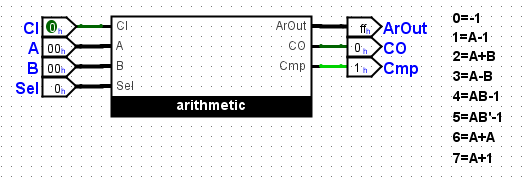
\includegraphics[width=\maxwidth{.95\linewidth}]{gfx/arith-06}
	\caption{Arithmetic Main Circuit}
	\label{fig:arith-06}
\end{figure}

This arithmetic device can be tested by entering numbers for the various inputs and checking to see if the output is correct. For example, if input \textit{A} was set to 3 and input \textit{B} were set to 4, then if \textit{Sel} is set to 2, \textit{ArOut} should be seven ($ 3+4 $). A test vector file has been provided for this lab so students can use that file to exercise all of the various settings in the circuit.

\section{Deliverable}

To receive a grade for this lab, complete the circuit. Be sure the standard identifying information is at the top left of the \lstinline[columns=fixed]|main| circuit, similar to: 

\bigskip
% The minipage environment keeps the three lines together - no page break.
\begin{minipage}{\linewidth}
	\begin{verbatim}
	George Self
	Lab 03: Arithmetic Operations
	September 17, 2019
	\end{verbatim}
\end{minipage}
\bigskip

Save the file with this name: \emph{\texttt{Lab03\_Arithmetic}} and submit that file for grading.

